\documentclass[12pt,a4paper,titlepage]{article}

\usepackage[utf8]{inputenc}
% Set level to number headings on
% part = -1
% chapter = 0
% section = 1
% subsection = 2
% subsubsection = 3
% paragraph = 4
% subparagraph = 5
\setcounter{secnumdepth}{0}

% Table of contents level if added
\setcounter{tocdepth}{2}

% Header and footer specifications
%\usepackage{lastpage}
\usepackage{fancyhdr}
\pagestyle{fancy}

\headheight = 28pt
\lhead{Sensor data aggregation through CoAP\\
\texttt{Work in progress}}
%\rhead{\thepage\ of \pageref{LastPage}\\} // Requires LastPage latex module
\rhead{} % Remove to enable Section name in the header
\cfoot{}
\rfoot{}

% Images
\usepackage{graphicx}

%%%%%%%%%%%%%%%%%%
% Custom new commands
%%%%%%%%%%%%%%%%%%

% From http://en.wikibooks.org/wiki/LaTeX/Title_Creation
% Used for the title page
\newcommand{\HRule}{\rule{\linewidth}{0.5mm}}

% Start of our document
\begin{document}

%Start page numbering from first page
%\thispagestyle{empty}
%\end{titlepage}
\setcounter{page}{2}

%Include the different parts in the lab report
% EXAMPLE: Sections and Paragraphs
% \section		- Level 1
% \subsection		- Level 2
% \subsubsection	- Level 3
% \paragraph		- Level 4
% \subparagraph		- Level 5 
% \section{<NAME_OF_SECTION>}

% EXAMPLE: Include graphics 
% \includegraphics[width=130mm,height=108mm]{intro4.png}

% EXAMPLE: Nested list
%\begin{enumerate}
%\item Nested list
%\begin{enumerate}
%\item
%\item
%\item
%\item
%\item
%\end{enumerate}
%\end{enumerate}


%%%%%%%%%%%%%%%%%%%%%%%%%%%%%%%%%%%%%%%%%
% Basic title page structure copied from 
% http://en.wikibooks.org/wiki/LaTeX/Title_Creation
%
% Christoffer Holmstedt on the 
% 17th of february 2012
%%%%%%%%%%%%%%%%%%%%%%%%%%%%%%%%%%%%%%%%%
\begin{titlepage}
\begin{center}

% Upper part of the page
% TODO ADD GRAPHIC
%\includegraphics[width=0.15\textwidth]{./logo}\\[1cm]    
\textsc{\LARGE Luleå University of Technology}\\[0.5cm]
\textsc{\Large Third year project}\\[0.5cm]

% Title
\HRule \\[0.4cm]
{\huge Sensor data aggregation through CoAP}\\[0.2cm]

\HRule \\[1.5cm]

% Author and supervisor
\begin{minipage}[t]{0.5\textwidth}
\begin{flushleft} \large
{\bfseries \emph Authors:}\\
Sophia \textsc{Bergendahl}\\
\emph{sopber-8@student.ltu.se}\\[0.2cm]
Edvinn \textsc{Bruun}\\
\emph{edvbru-9@student.ltu.se}\\[0.2cm]
William \textsc{Gustafsson}\\
\emph{wilgus-9@student.ltu.se}\\[0.2cm]
Christoffer \textsc{Holmstedt}\\
\emph{cihhol-7@student.ltu.se}\\[0.2cm]
Marcus \textsc{Rådman}\\
\emph{marrdm-9@student.ltu.se}\\[0.2cm]
Kristoffer \textsc{Svensson}\\
\emph{kirsev-9@student.ltu.se}\\[0.2cm]
Ludwig \textsc{Thurfjell}\\
\emph{ludthu-7@student.ltu.se}\\
\end{flushleft}
\end{minipage}
\begin{minipage}[t]{0.45\textwidth}
\begin{flushright} \large
{\bfseries \emph Supervisors:} \\
Ulf \textsc{Bodin}\\
\emph{ulf.bodin@ltu.se}\\[0.2cm]
Jens \textsc{Eliasson}\\
\emph{jens.eliasson@ltu.se}\\[0.2cm]
Rumen \textsc{Kyusakov}\\
\emph{rumen.kyusakov@ltu.se}\\[0.2cm]
\end{flushright}
\end{minipage}

\vfill

% Bottom of the page
{\large \today}

\end{center}

\end{titlepage}

% EXAMPLE: Sections and Paragraphs
% \section		- Level 1
% \subsection		- Level 2
% \subsubsection	- Level 3
% \paragraph		- Level 4
% \subparagraph		- Level 5 
% \section{<NAME_OF_SECTION>}

% EXAMPLE: Include graphics 
% \includegraphics[width=130mm,height=108mm]{intro4.png}

% EXAMPLE: Nested list
%\begin{enumerate}
%\item Nested list
%\begin{enumerate}
%\item
%\item
%\item
%\item
%\item
%\end{enumerate}
%\end{enumerate}

\section{Project Description}
\subsection{Background}
Luleå University of Technology conducts research on lowpower wireless microprocessors called "Mulle". 
These microprocessors can be used for various things depending on which type of sensors you connect to it, everything from measuring temperature or vibrations in a car to analyzing the quality of the road that you drive on.

Every year northern parts of Sweden are used for testing cars during winter conditions.
First you decide what you want to test in the car, then you do this by placing local sensors within the car.
When enough data is collected you return back home.
At the testing facility the data is now available for analysis.
Depending on the results from the previous runs you might want to test some parts in more detail so you re-configure all sensors and go out for another test run.

This process is time consuming when you need to return to testing facility to be able to analyze and re-configure all sensors.
In todays society most computers are connected to internet and/or other private networks, most of these computers have the ability to be remotely configured and maintained.
The goal with the project is to be able to analyze data from sensors in realtime and re-configure them on the fly while testing is in progress.
\subsection{Project Targets}
\begin{enumerate}
\item Be able to send live sensor data from multiple "Mulles" to an online logging server/service.
\item Be able to read sensor data on the web with both a PC (web browser) and through an Android mobile device.
\item Be able to re-configure the sensors through a web interface and through an Android mobile device.
\end{enumerate}

\subsection{Technical limitations}
The technical limitations for this project was mainly to restrict how flexible the finished solution was.
The Mulles can be used together with any kind of sensors.
In this project the main goal was to get it operational in a car and measure temperature and some other variables.


%TODO: Vad har explicit uteslutits från arbetet?

% EXAMPLE: Sections and Paragraphs
% \section		- Level 1
% \subsection		- Level 2
% \subsubsection	- Level 3
% \paragraph		- Level 4
% \subparagraph		- Level 5 
% \section{<NAME_OF_SECTION>}

% EXAMPLE: Include graphics 
% \includegraphics[width=130mm,height=108mm]{intro4.png}

% EXAMPLE: Nested list
%\begin{enumerate}
%\item Nested list
%\begin{enumerate}
%\item
%\item
%\item
%\item
%\item
%\end{enumerate}
%\end{enumerate}

\section{Execution of the project}
\subsection{Scrum and how it has been used}
It was decided back in november that the entire project would be divded into three sprints.
The exact dates were to be decided in the beginning of each sprint.
In cooperation with the client the scope of the project and the scope of the first sprint was decided upon in november.
During the first projectmeeting the first sprint goal was divided into eight sprint stories.
It soon became clear that those eight stories were way to big, at the end of the sprint none of the stories had been finished.

Lesson learnt, the second sprint was divided into smaller stories which gave immidiate result when the first 69 sprint story points finished during the second sprint.

To decide upon size for each sprint story, for the second and third sprint, "planning poker" \cite[p.~42]{kniberg07} was used.
For every sprint story each project member wrote down an estimate on the scope for each story.
With planning poker it became clear that each project member had a different vision for each story.
A short discussion after each estimate made it more clear on how big the scope was, an agreement was usually made within a few minutes.

%
% TODO: Skriv hur vi har använt Scrum och relatera till våra referenser \cite{kniberg07}
%
\subsection{One project, three sprint goals}
As mentioned earlier the project was divided into three sprints.
This meant that three different sprint goals had to be divided into smaller sprint stories which in turn had to be assigned to a project member.
Due to all project members being new to most of the tasks at hand the first team division was made with focus on components \cite[p.~106]{kniberg07}.
The goal with this was that each smaller team within the project could sit together and dive deep into their specific part such as the Mulle, the server parts or the android code.
Later on a split into cross-component teams \cite[p.~107]{kniberg07} was aimed for but due to some persistent bottlenecks in some components this was never done.

For all sprints the sprint planning meeting were used to categorize each sprint story into the different components (Mulle, Server, Android).
It was then up to each component based team to split their stories between themselves.
This ended being a very flexible solution, in some cases, to flexible when a team didn't use the Scrumboard online at Scrumdo.com the team could wander off from the sprint story they were supposed to work on.
For the last sprint everyone got at least one sprint story assigned to themselves directly during the sprint planning meeting.
This was made to put more focus on using the Scrumboard at Scrumdo.com.

A move to cross-component teams was never made instead an attempt to increase speed for the Mulle and the Android component was made by moving one team member from the server team to the Mulle team and another to the Android team.
The server component at this time was way ahead of the other components.
Another week later it became clear that the additional team member for Mulle team was not needed, cause the problem was still a bottleneck that only one or two team members could work on at a single point in time, a move back to the server team was made.

\subsection{Individual time monitoring and speed}
\subsubsection{Sophia Bergendahl}
\subsubsection{Edvin Bruun}
\subsubsection{William Gustafsson}
\subsubsection{Christoffer Holmstedt}
Exempelvis kan lista användas om man vill. Jag, christoffer, kommer inte använda det tror jag.
\begin{enumerate}
\item TODO: Hur man citerar till specifik sida i kurslitteraturen. \cite[p.~42]{kniberg07}
\item TODO: Hur man citerar utan sidhänvisning \cite{kniberg07}
\item Third sprint story
\end{enumerate}
\subsubsection{Marcus Rådman}
\subsubsection{Kristoffer Svensson}
\subsubsection{Ludwig Thurfjell}
\subsection{Reflection about Scrum usage during this project}
Alot has been learnt during this project and to keep it short the following lessons learnt and improvements that can be made are a chosen few.

At the end of all projects when the deadline is closing in the pace of the development often increases.
A downfall of this is that when the speed increases the quality of the code often decreases.
Scrum is a solution to this problem with the main goal of keeping a steady development pace and always keeping the quality of the code as good as possible above some minimum criteria.
With to long sprints, projects will still end up with a big deadline, this is what happened in this project.
In total the project lasted about 17 weeks including the winter holidays.
Instead of three sprints where each lasted about five weeks a project split into smaller sprint would have been better.
If time travel was possible this project would have had two smaller sprints in the beginning each would have lasted for two weeks.
The first sprint with goal of configuring all required software for everyone such as setting up git, the different IDEs, gcc and other required software/tools.
The second sprint with the goal of understanding what was available at the time and get all basic functionality working.
If the project had found any big bottlenecks at the end of the second sprint that would be the point in time to halt the project and really rethink what to focus on.
The remaining weeks should have been divided into three evenly sized sprints.

Another big improvement could have been made in the relation between Scrum team and product owner.
From the beginning it was unclear who was the product owner out of three supervisors/clients, this should have been defined to one single person as early as possible before continuing with any other work.
The absence of the product owner before and during our sprint planning meetings resulted in alot of confusion when it was up to the team to decide an estimate for each sprint story.
The lesson learnt from this is that without a product owner the scrum team will fumble in blindness forever or as Kniberg writes \cite[p.~25]{kniberg07} {\em "...each story contains three variables that are highly dependent on each other"}.
There is no way the team can choose a good estimate when there is no product owner that has already chosen an importance and scope for each sprint story to start with and is available to change that during the course of a sprint planning meeting.

The last and perhaps the most important improvement that will be mentioned is the importance of having a team member taking the role as Scrum master.
Without the Scrum master during the first sprint everyone was on their own.
For the second and third sprint the Scrum master role was appointed to one team member.
This improved the communication within the Scrum team alot and also made it possible for individual team members to have someone to go to in case of general questions and/or other problems.

TODO: ...samt redovisning av arbete med krav mot kravställare och hantering av projektvariablerna omfattning och kvalité.
%
% Andra kommentarer som kan vara värda att ta med om Scrum och hur det 
% har använts i detta projekt.
%
%TODO: Tydligare sprint mål för varje sprint från kravställare. En mening som beskriver syftet med respektive sprint.
%TODO: Tydligare demo av varje punkt
%TODO: Vi skulle ha satt ner foten på hur många delar vi skulle jobba med samtdiigt. Startat med Mulle och Server enbart...sedan android i mån av tid för att få mer fokus i projektet, vi var trots allt bara sju personer.
%TODO: Ingen "experthjälp" med android tillgänglig. I detta läge gör det stor skillnad om man är två, tre eller fyra. Varje programmerare ökar hastigheten med mer än bara sin tid hen kan lägga till eftersom felsökning oftast går betydligt snabbare för fler personer än enbart två. Många fel beror också på utvecklingsmiljön, om man är fler med samma miljlö så är det större chans att någon har stött på problemet tidigare och har en lösning.
%TODO: Reflektion över flytten av individuella team members server till mulle och android. Väldigt "dyrt" i uppstartskostnad.

% EXAMPLE: Sections and Paragraphs
% \section		- Level 1
% \subsection		- Level 2
% \subsubsection	- Level 3
% \paragraph		- Level 4
% \subparagraph		- Level 5 
% \section{<NAME_OF_SECTION>}

% EXAMPLE: Include graphics 
% \includegraphics[width=130mm,height=108mm]{intro4.png}

% EXAMPLE: Nested list
%\begin{enumerate}
%\item Nested list
%\begin{enumerate}
%\item
%\item
%\item
%\item
%\item
%\end{enumerate}
%\end{enumerate}

\section{Results}
\subsection{Deliverables}
Mainly due to being unable to setup communication from the Mulle to the server, project target number one listed in the beginning of this document is not met.
What is delivered from the project concerning this is available in Appendix A where a guide on how to get started where this project ends is available.

Project target number two is not met.
What is delivered from the project is a basic webapplication with a simple database structure as the back-end where future real sensor data can be stored.

Project target number three is not met.
Basic functionality on how to use EXI as encoding for sensor data is available for the Mulle and the Android application but hasn't been tested.
No work on EXI has been made for the server though there exist a simple webpage to turn a value on or off.

\subsection{Testing}
During this project testing has been made by each project member.
The scope of the testing for each story has been up to each project member to decide upon.
Right before each sprint demo a project meeting was scheduled were each one showed what was completed and what was not.
Depending on what was ready at that point in time the entire Scrum team decided what was going to be presented at the demo and a test was made to confirm that it was possible to show the parts that were decided upon.
No further testing was made during this project.
\subsection{Lessons learnt}
Communication is always troublesome, it's usually easy to get a system to transmit data and another to do the same.
The hard part is when you want different system to actually communicate with each other.
This boiles down to the lesson learnt that the project should have focused more on specific components instead of spreading out on all three components (Mulle, Android and the server) from the beginning.
The goal should have been to get the Mulle communicate with either the server or the android device to start with.
When that was operational new systems could have been added to the mix.

Testing is always hard to do, it might be easy to test specific test cases but is very hard to test all possible usages.
To make sure that your codebase doesn't become useless in the long run you need somekind of automated testing to make sure that all previous bugs found is tested automatically with all new improvements and add-ons.
It might be time consuming in the beginning of a project but it's priceless in the end.
An important part of testing is to test both individual components and interaction between different components.
If only testing is made to the interaction between different components a finished component cannot be tested until the other one is finished aswell, this creates bottlenecks for the entire project.

When is something done?
Do not let this question be up to the individual programmer, it puts the programmer in a difficult situation.
Either the programmer wants to create the perfect spot and keeps going forever or the programmer will take shortcuts that will comeback and haunt you later on.
It must be up to the team to decide when something is done or not.
This will make it alot easier in the day to day work for everyone, if anybody is uncertain if it's completed or not, just look into what was decided earlier.
\subsection{Suggested improvements}
Without meeting any of our project targets it's hard to suggest improvements except the obvious one to complete what has been started. 
Instead of going straight at it and try to finish it all as soon as possible some thought process need to be put into the question, what really needs to be finished?
% TODO: Fortsätt på Mullen
% TODO: Tänk efter om CoAPy är rätt väg att gå
% TODO: Skippa android tillsvidare om den inte är viktigare än servern.

%
% Scrum och relatera till våra referenser \cite{kniberg07}
% \cite[p.~107]{kniberg07}
%

% EXAMPLE: Sections and Paragraphs
% \section		- Level 1
% \subsection		- Level 2
% \subsubsection	- Level 3
% \paragraph		- Level 4
% \subparagraph		- Level 5 
% \section{<NAME_OF_SECTION>}

% EXAMPLE: Include graphics 
% \includegraphics[width=130mm,height=108mm]{intro4.png}

% EXAMPLE: Nested list
%\begin{enumerate}
%\item Nested list
%\begin{enumerate}
%\item
%\item
%\item
%\item
%\item
%\end{enumerate}
%\end{enumerate}

\section{Conclusions}


% EXAMPLE: Sections and Paragraphs
% \section		- Level 1
% \subsection		- Level 2
% \subsubsection	- Level 3
% \paragraph		- Level 4
% \subparagraph		- Level 5 
% \section{<NAME_OF_SECTION>}

% EXAMPLE: Include graphics 
% \includegraphics[width=130mm,height=108mm]{intro4.png}

% EXAMPLE: Nested list
%\begin{enumerate}
%\item Nested list
%\begin{enumerate}
%\item
%\item
%\item
%\item
%\item
%\end{enumerate}
%\end{enumerate}

\begin{thebibliography}{9}

\bibitem{kniberg07}
    Henrik Kniberg,
    \emph{Scrum and XP from the Trenches}.
    C4Media Inc, Publisher of InfoQ.com,
    978-1-4303-2264-1,
    \texttt{http://infoq.com/minibooks/scrum-xp-from-the-trenches},
    2007.

\end{thebibliography}

% EXAMPLE: Sections and Paragraphs
% \section		- Level 1
% \subsection		- Level 2
% \subsubsection	- Level 3
% \paragraph		- Level 4
% \subparagraph		- Level 5 
% \section{<NAME_OF_SECTION>}

% EXAMPLE: Include graphics 
% \includegraphics[width=130mm,height=108mm]{intro4.png}

% EXAMPLE: Nested list
%\begin{enumerate}
%\item Nested list
%\begin{enumerate}
%\item
%\item
%\item
%\item
%\item
%\end{enumerate}
%\end{enumerate}
\section{Appendix A - How to build upon the codebase}
This appendix include information on how to build upon our codebase for the Mulle (C), server code (Python, PHP/HTML5 and C) and Android Mobile phone (Java).
\subsection{Mulle}
The Mulle communication via COAP is far from finished and therefore here is a guide how to get started followed by what should be further built. The instruction on how to get started are done in Ubuntu, the versions that were tested are 10.04 and 11.10. Windows or any other OS will not be covered in this guide.

The Mulle software required is all in the Software-PAN-NAP folder which contain necessary libraries and applications. It is assumed that you have acquired this because it's essential for any development.

\subsubsection{Getting started}
The first step you will take is to download the code from a repository on Github.com, if you don't know how to do this there are several guides how to do that on their site. Since there are several ways to do this here are the links to the repository:
\begin{itemize}
\item Download zip: \url{https://github.com/christofferholmstedt/vehicletesting/zipball/master}
\item Git: \url{git://github.com/christofferholmstedt/vehicletesting.git}
\item SSH: \url{git@github.com:christofferholmstedt/vehicletesting.git}
\end{itemize}
When you've done this note that you'll only need files from the ../vehicletesting/code/Mulle folder.
In this folder there are two subfolders named Coap and PAN-Router\_demo. 
These two folders are going to seperate locations in your Mulle software folder, 
since the Coap folder contains the code for the protocol and PAN-Router\_demo code for the application. 

The folder Coap should be copied into ../$<$Mulle Software folder$>$/Libary/misc/apps/ 
and the PAN-Router\_demo folder goes to  ../$<$Mulle Software folder$>$/Applications/. 
The PAN-Router\_demo folder is optional to use, if you want to use you're own Mulle program you need to include coap.h and run coap\_init() somewhere in your applications c-file. 
Since the coap-protocol isn't official you also need to put a "\#define LWIP\_COAP" and set it to 1 in proj\_arch.h(as well as turn off any other protocol that are used for communcation) 
and finally you need to add coap.c in the SOURCES.mk file. This is done by adding "\$(LIBDIR)/misc/apps/coap/coap.c" to the LWIP\_Apps field.

Now when you have the code set up you must install the gcc compiler, namely m32c-elf-gcc, for this type of hardware. Do the following steps in your terminal with sudo, alternatively make a script. Be prepared to redo this if you're doing it in a script. It's preferable to do this step by step because it has a higher rate of succeeding. 

Alternatively you can follow this guide(however, it's strongly advised not to): \url{http://www.eistec.se/docs/wiki/index.php?title=Mulle\_software\_with\_GCC}

Setup Development Host:
\begin{itemize}
\item apt-get install build-essential
\item apt-get install m4 autoconf libtool gawk bzip2 bison flex gettext texinfo zlib1g-dev 
\item apt-get install libmpc-dev libmpfr-dev
\end{itemize}

\noindent When this is done you need to download binutils and install it:
\begin{itemize}
\item wget \url{http://ftp.gnu.org/gnu/binutils/binutils-2.19.1.tar.bz2}
\item tar xjf binutils-2.19.1.tar.bz2
\item mkdir binutils-obj
\item cd binutils-obj
\item ../binutils-2.19.1/configure --target=m32c-elf
\item make
\item sudo make install
\item cd ..
\end{itemize}

\noindent In the next step you'll download gcc-4.3.3 and newlib 1.17 and install them:
\begin{itemize}
\item wget \url{ftp://ftp.nluug.nl/mirror/languages/gcc/releases/gcc-4.3.3/gcc-4.3.3.tar.bz2}
\item wget \url{ftp://ftp.nluug.nl/mirror/languages/gcc/releases/gcc-4.3.3/gcc-core-4.3.3.tar.bz2}
\item wget \url{ftp://sources.redhat.com/pub/newlib/newlib-1.17.0.tar.gz}
\item tar xjf gcc-4.3.3.tar.bz2
\item tar xjf gcc-core-4.3.3.tar.bz2
\item tar xzf newlib-1.17.0.tar.gz
\item cd gcc-4.3.3
\item ln -s ../newlib-1.17.0/newlib
\item ln -s ../newlib-1.17.0/libgloss
\item cd ..
\item mkdir gcc-obj
\item cd gcc-obj
\item ../gcc-4.3.3/configure --target=m32c-elf --with-newlib --enable-languages="c"
\item make
\item sudo make install
\item cd ..
\end{itemize}
When you've done all these steps you should try typing this into your terminal: "m32c-elf-gcc --version" and check that it says "m32c-elf-gcc (GCC) 4.3.3" just to be sure.

Now you're good to go, a final note on how get get set up is how to push your code onto the Mulle. Pushing your programs is done in a few steps, first you need to orient your way to the folder containing the program you're pushing in the terminal, then do these steps:
\begin{itemize}
\item make clean
\item make all
\item make program
\item make debug
\end{itemize}
The “make clean” is only needed if you changed something in the system files and when running “make program” the Mulle must be set to “Program Mode”. If all your modified files are correct your code will be pushed to the Mulle, if you get a “Clock Validation Error” make sure the Mulle is set to “Program Mode” and try again. The “make debug” command starts mulle\_term, which is a terminal debugger for the Mulle, so when you put it back on “Run Mode” you'll see what it is doing(in the form of printouts).

\subsubsection{Further developement}

You will need some sort of device that can share internet through Bluetooth to the Mulle, whether it be a telephone or a personal computer with an USB-dongle. To test COAP protocol, you can download the Copper addon for Firefox. The coap\_init() function in coap.c initializes so that when you receive UDP packets on the Mulle the function coap\_input() is run.

First the coap\_input() function needs to be properly made, since it does nothing useful at this time. What needs to be done is that the function should put all the correct values into a coap struct and based on what values are in each field the function should decide where to send the infomation next for handing. 

A suggestion for handling the COAP payload is by working with EXIP. You create and decode exi files directly on the mulle. EXI-files which have the same structure as XML are interesting for this type of projects since it's light and you can easily write scripts with XML structure.

You can find out more about EXIP here: http://exip.sourceforge.net/ .
A final suggestion is to finish the debug\_coap\_print() function since it will be very helpful for debugging.

\subsection{Server}
\subsubsection{Coapy server}
\paragraph{Existing implementation}
The server is based on CoAPy, which is a python implementation of the CoAP protocol. The actual server implementation is a modification of the example server provided along with CoAPy.
Some minor changes were made to it allowing it to accept all forms of CoAP messages, provided they are taken care of properly. We also added a way for new services to be easily added 
and used. 

The procedure when adding new services is as follows:
\begin{enumerate}
\item Create a new .py file with the name corresponding to the actual service name (e.g. "TestService.py") in the "services" directory
\item The file should contain only the necessary imports (including CoAPy parts) along with a class name the same thing as the file ("TestService", in this case)
\item The class is to define a single function "process" in which the actual actions of the service are to be made
\end{enumerate}

Using an existing service, like "CounterService.py", is highly recommended for understanding how a service should be structured and laid out.

\paragraph{Further development}
The server itself should be set to add new services for operation. What needs more work is the incorporation of a few things:

\begin{enumerate}
\item An actual XML scheme for configuration of mulle nodes. This point is not particular to the server, however.
\item Implement ways for the server to make use of the EXIP application to translate the XML that's to be sent into EXI via the command line.
\item Make services corresponding to the functionality you would like to have for configuration and communication with mulles and android devices, respectively.
\end{enumerate}
\subsubsection{Webpages and database}
 
The webpages and database consists of Apache2 which is an web server, MySQL which is a database management system and PHP which is a language for producing dynamic webpages.
LAMP (Linux), WAMP (Windows) or MAMP (Mac) can be used to build a web server it is an web-platform that consists of Apache, MySQL and PHP.

\paragraph{Webpages}

The webpages are built up using mulleheader.php which contains the header and sidebar, a .php file containing page content and mullefooter.php which contains the footer.

We have built two webpages using this concept; One that shows information from the database and its .php file that holds page content is mulledatabase.php and one consists of 
a php form to turn on or off a lamp and its .php file that holds page content is mullebuttons.php. The mullebuttons.php also contains a call to a .py file called testsender.py
that with some work can run a service on the CoAP server.


How to create a new webpage:

1. 	Create a new .php file for page content

2. 	In the top of the .php file print:\\$<?$php include("mulleheader.php"); $?>$

3. 	Between \\$<$ section id ="main" $>$ and $<$/section $>$ write the page content

4. 	In the bottom of the .php file print \\$<?$php include("mullefooter.php"); $?>$

\paragraph{Database}

We created a MySQL database and named it mulle and to this database we added two tables one that keeps track of communication on server and one that keeps track of connected/active 
devices. Online you can find many guides on how to add to a LAMP, WAMP or MAPM MySQL database, but down below shows some commands good to know when creating a database.  


How to create a new database:

1. 	Open up your MySQL Console and login

2. 	mysql$>$ \texttt{SHOW DATABASES;}

3. 	mysql$>$ \texttt{CREATE DATABASE the_database_name;}

4. 	mysql$>$ \texttt{USE the_database_name}

5. 	\texttt{CREATE TABLE name_of_table (name_first_column_in_table VARCHAR(20), name_second_column_in_table VARCHAR(20), name_date_and_time DATETIME);}
	This creates a table with three columns.
	
6. 	\texttt{SHOW TABLES;}

7. 	\texttt{EXPLAIN name_of_table;}

\subsection{Android Mobile Phone application}

The primary goals for the android applications were to;
%communication goes via a server.
\begin{itemize}
 \item communicate using CoAP over an UDP connection
 \item encode the sent packets with EXI to reduce the size of packets
 \item have a graphical UI capable of controlling multiple devices.
\end{itemize}
% UNDERSÖK OM MER SKA IN HÄR

\subsubsection{The goal of the finished product}

The application starts off by showing the server menu. One will have to either add a server or use a saved one. 
Clicking on a server in the list will cause the application to validate that the server is alive and thereafter it will perform a CoAP discovery on the server. 
When receiving an answer to the discovery the application will start filling the device menu with devices and their services. The device menu can then be accessed to use the services available.
The services generally works as follows: The application gets a click on the chosen service, so it sends its message to the service owner, whereafter the services device either changes something or responds.
The service owner will then have to respond to the Android application with the updates made, this can be with a confirmation or a whole new CoAP message. This makes the application respond by updating the GUI with the new values.\smallskip

The pre-built services are generalized to: 
\begin{itemize}
\item IsOn, provides an item with a checkbox that is checked if a service is on (for example a lamp). Clicking on this should provide a change on the selected device.
\item GetValue, provides an item which shows the last value provided. Clicking on the item should provide an update.
\item SendValue, provides an item which have a view of the current value and a textbox where one can send a payload to the device.
\end{itemize}

Another feature of the finshed product would be the options menu where the application will allow things like turning EXI encoding on or off. 

\subsubsection{What exists today}

Today there exists a communication part which allows one to send and recieve CoAP messages. This part uses a library made out of \texttt{jCoAP revision 202b8f8eb7b4, http://code.google.com/p/jcoap/}%s.unger.mobil@gmail.com committer ,	chr.lerche@gmail.com	owner,	nic@nclm.de	owner 
to get the CoAP features. The reason for making this a library is to make a Java project compile in the Android project without complications. The jCoAP project is not yet finished but the features requested for this application is present. The EXI converter is currently not available but is planned to use exificient, 
which can be found at \url{http://exificient.sourceforge.net/}.

The GUI is another important part of the application. It is built to be able to controll multiple servers and devices. 
To make this possible the application has 3 tabs:	%the default thought was to have a checkbox in the server menu to allow one to decide whether a server is being currently used, this idea has however been dropped due to lack of time.
\begin{itemize}
 \item Device tab
 \item Server tab
 \item Options tab
\end{itemize}

The Options tab does currently not contain anything but should simply allow a user to change things about how the application should work and what and how things should be displayed. 

\begin{center}
 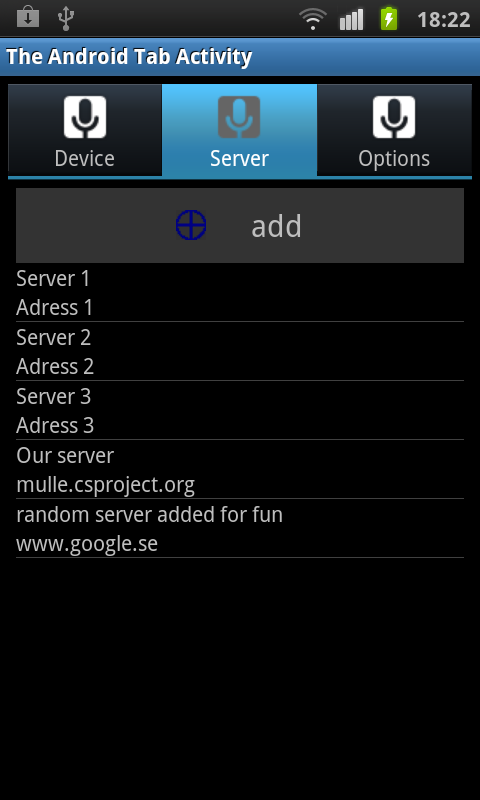
\includegraphics[scale=0.25]{android-server.png}%\caption{The Server tab of the Android application}
\end{center}
 \\The Server tab shows all the active servers. You can click on the add button in the server menu and a window appears where you write in the name and adress appear. The servers then appears in a listview where it's easy to keep track of them. In the future this can be complemented with a network discovery of nodes, however, my personal opinion is that it should be possible to manually add an server.

\begin{center}
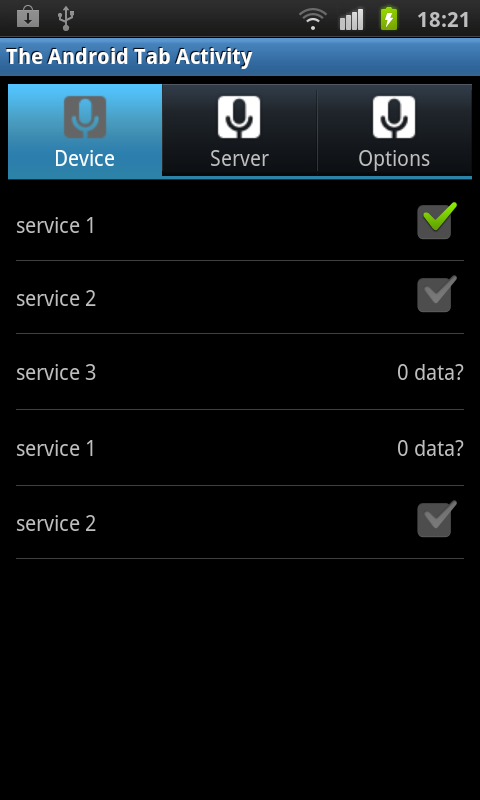
\includegraphics[scale=0.25]{android-device.png}%\caption{The device tab of the Android application}
\end{center}
\\The Device tab is the latest addition in the GUI and contains the actual services that are available. It contains a custom ArrayAdapter that have been tweaked to be able to display children of the interface rowdata.
In it's current state it is possible to add items to this list in the code by calling the NewItem() function with proper parameters. If the prebuild service types would not suffice it's relatively easy to add new ones.
Simply extend the rowdata() interface and create the desired xml for the item, do not however forget to add a typenumber for the NewItem() function to be able to create it. 
This also allows the children to define for their own what should happen if clicked, updated and so on.


\end{document}
